\documentclass[a4paper, 12pt]{paper}

\usepackage[utf8]{inputenc}
\usepackage[T1]{fontenc}
\usepackage{gensymb}
\usepackage{graphicx}


\author{Florian Reinhard}

\begin{document}

\title{Smoothing Station}
\maketitle

\begin{figure}[h]
    \centering
    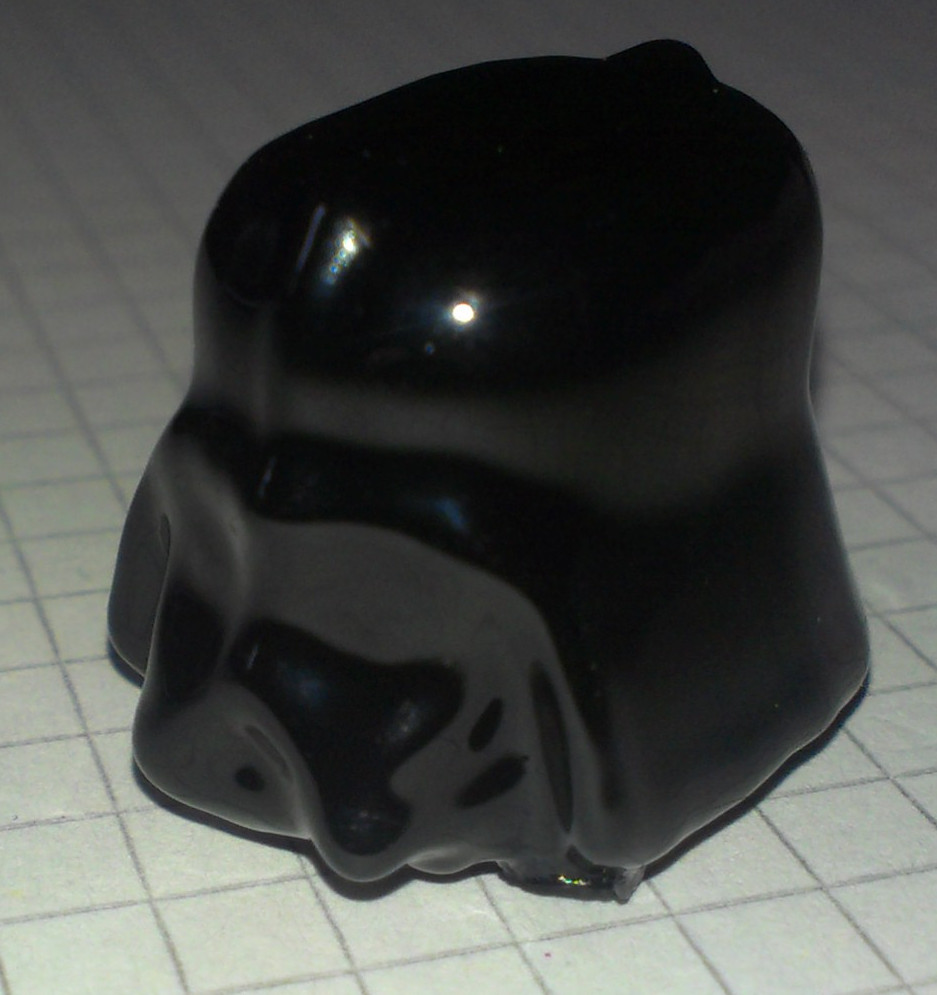
\includegraphics[width=0.6\linewidth]{vader.jpg}
\label{fig:title}
\end{figure}

\section{Basic functionality}
The \emph{Smoothing Station} is used to smooth the surface of a part made out
of polymers by exposing it to a vaporized solvent for a few minutes.
To expose the part to a constant atmosphere (i.e.\ constant temperature,
concentration, and pressure), a pump creates a constant flow of vapor around
the object. Two valves allow for the pump to change between pumping vaporized
solvents or fresh air. This increases the abruptness at which the reaction can
be started or stopped.

\section{Part list}

\subsection{High level}
\begin{itemize}
    \item Hot plate and stirrer (closed-loop, up to $100\,^{\circ}\mathrm{C}$)
    \item Solvent container
    \item Pump (chemical grade)
    \item Transparent sample container (chemical grade)
    \item PTFE tubing ($\approx2.5\mathrm{m}$)
    \item Three-port valve ($\mathrm{2x}$)
\end{itemize}

\begin{figure}[h]
    \centering
    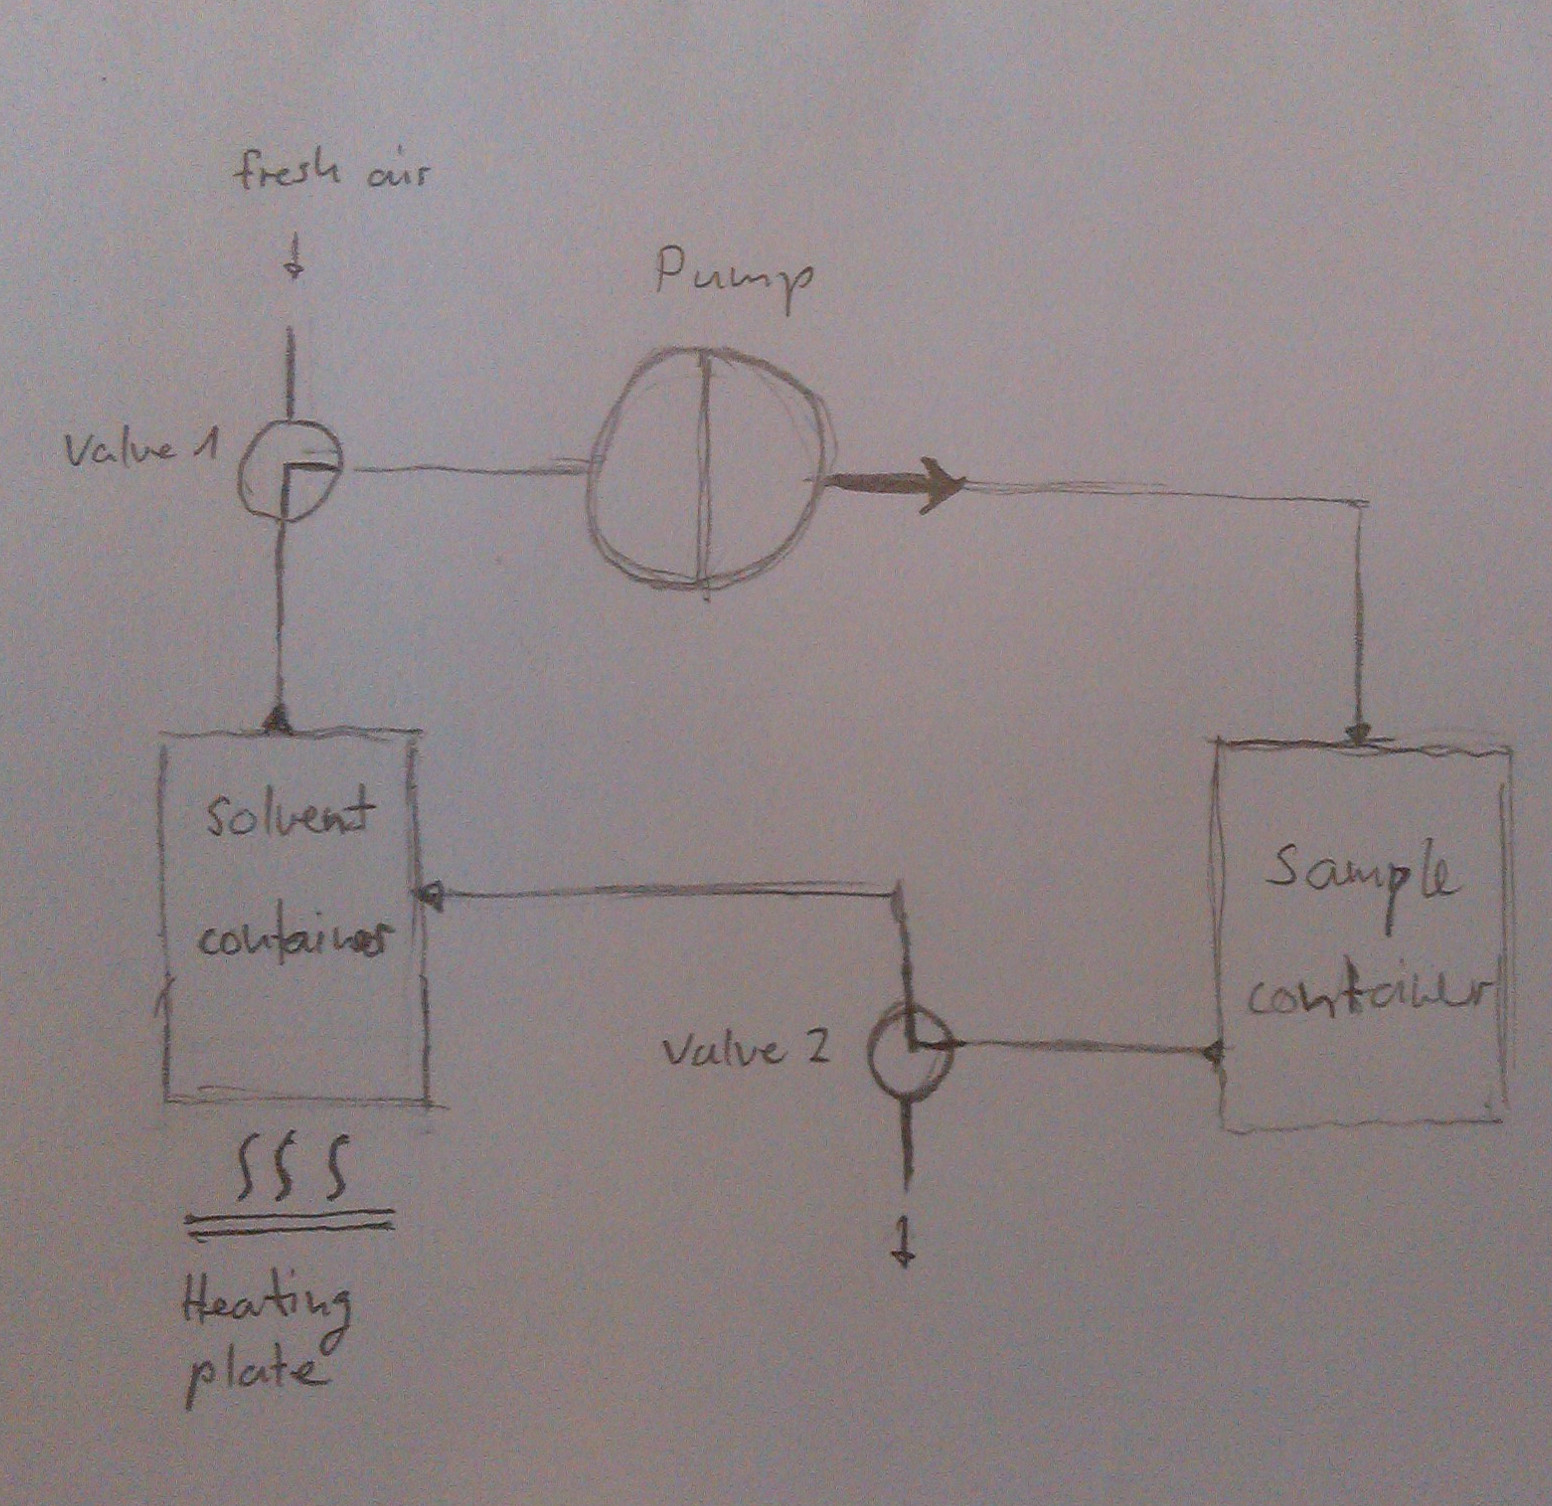
\includegraphics[width=0.9\linewidth]{schematics.jpg}
    \caption{Schematics of the basic functionality.}
\label{fig:schmeatics}
\end{figure}

\section{Critical points}

\subsection{Mechanical}
\paragraph{Sample holder}
The sample needs to be held in the vapor stream. The sample holder should at
the same time
\begin{itemize}
    \item keep the sample in place
    \item touch the sample the least possible
    \item not disturb the vapor stream
    \item prevent the accumulation of condensed solvent around the sample
    \item not leave deep marks on the sample surface.
\end{itemize}

A possible solution is a fine wire mesh, placed a couple of centimeters above
the bottom of the sample container.

\paragraph{Sample container}
The sample is put in a transparent container, so it can be observed visually
during the smoothing process. There are a couple of critical points:
\begin{itemize}
    \item it should be a simple manipulation to open the container and change
        the sample
    \item the \emph{inlet} needs to be placed at the \emph{top} of the container
        and connected to a tube
    \item the \emph{outlet} needs to be placed at the \emph{bottom} of the
        container and connected to a tube
    \item the vapor stream shouldn't be pointed directly at the sample to ensure
        a homogeneous smoothing of the surface
    \item condensed solvent should be collected in a controlled manner
\end{itemize}

\paragraph{Solvent container}
The solvent is being vaporized on a hotplate and stirred at the same time for
better control and thus should be put in a suitable container, e.g.\ a conical
flask. While there's an outlet for the produced vapor, there's also an inlet
for the used vapor coming back from the \emph{sample container}. These two
ports shouldn't be placed next to each other, to ensure a constant temperature
and concentration for the vapor leaving the container. A possible solution is
adding a tube to the \emph{inlet} going all the way down into the liquid solvent
at the bottom.



\end{document}
